\bookchapter{Motors}\label{ch:hw6}

\section*{Explanation}
Everything a robot does in the world, every step, every kick, is done by motors. A walking robot has twenty or more of them, each fighting gravity several times per second, and the choice and control of the motors decide how strong, fast, quiet, efficient and safe the robot is. This chapter explains the physics of the electric motor in a way that lets you \emph{calculate} with it: what a motor can do at which speed, why a gearbox is needed, how an H-bridge and PWM drive a motor, and how to check that a motor is big enough. Chapter~\ref{ch:hw7} then shows the special actuators of modern humanoids, and Part~\ref{part:control} how to control them.

\section*{How a motor works}
A current in a wire inside a magnetic field experiences a force (the Lorentz force); arranged around a shaft, this force becomes a \textbf{torque} $\tau$ (newton-metres, Nm). The same arrangement works in reverse: a coil that moves in a magnetic field has a voltage induced, the \textbf{back-EMF} that opposes the supply voltage. Both effects are proportional:
\[
\tau=k_t\,I\qquad\text{and}\qquad U_\text{emf}=k_e\,\omega,
\]
with the \textbf{torque constant} $k_t$ (Nm/A) and the \textbf{speed constant} $k_e$ (V per rad/s); in SI units $k_t=k_e=k$. The angular velocity $\omega$ is in rad/s ($1$\,rpm $=2\pi/60=0.105$\,rad/s). The electrical side is a resistor $R$ (the winding) in series with the back-EMF (Figure~\ref{fig:hw6_model}):
\[
U=R\,I+k\,\omega.
\]
\begin{center}
\begin{circuitikz}[scale=0.9,transform shape]
  \draw (0,0) to[battery1,l=$U$] (0,3) to[R,l=$R$] (3,3) to[american voltage source,l=$k\omega$,invert] (3,0) -- (0,0);
  \draw[->,thick,blue!60!black] (1.0,3.5)--(2.0,3.5) node[midway,above,font=\footnotesize]{$I$};
  \node[font=\footnotesize,anchor=west] at (4.2,2.3) {$\tau=k\,I$};
  \node[font=\footnotesize,anchor=west] at (4.2,1.6) {$U=R\,I+k\,\omega$};
  \node[font=\footnotesize,anchor=west] at (4.2,0.9) {$P_\text{el}=U\,I$,\ $P_\text{mech}=\tau\,\omega$};
\end{circuitikz}
\captionof{figure}{The equivalent circuit of a DC motor: winding resistance plus back-EMF.}\label{fig:hw6_model}
\end{center}
From these three lines follow all the properties of the motor.

\subsection*{The torque--speed line}
\begin{itemize}[nosep]
  \item \textbf{Stall} ($\omega=0$): no back-EMF, the current is largest, $I_s=U/R$, and so is the torque, $\tau_s=kU/R$.
  \item \textbf{No load} ($\tau=0$, so $I\approx0$): the motor speeds up until the back-EMF equals the supply voltage, $\omega_0=U/k$.
  \item In between, the speed falls \emph{linearly} with the load: $\omega=\omega_0\,(1-\tau/\tau_s)$.
\end{itemize}
Mechanical power $P=\tau\omega$ is a parabola with its maximum at half the stall torque and half the no-load speed: $P_\text{max}=\tau_s\omega_0/4$.
\begin{center}
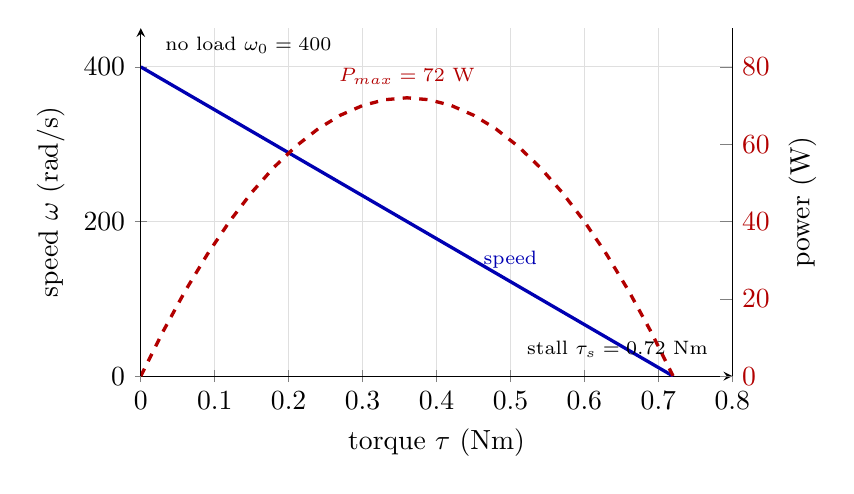
\begin{tikzpicture}
\begin{axis}[width=0.75\textwidth,height=6cm,xlabel={torque $\tau$ (Nm)},ylabel={speed $\omega$ (rad/s)},xmin=0,xmax=0.8,ymin=0,ymax=450,grid=both,grid style={gray!25},axis lines=left,xlabel near ticks,ylabel near ticks,
 axis y line*=left, axis x line*=bottom]
  \addplot[blue!70!black,very thick,domain=0:0.72]{400*(1-x/0.72)};
  \node[font=\scriptsize,blue!70!black] at (axis cs:0.5,150) {speed};
  \node[font=\scriptsize,anchor=south west] at (axis cs:0.02,405) {no load $\omega_0=400$};
  \node[font=\scriptsize,anchor=south east] at (axis cs:0.78,12) {stall $\tau_s=0.72$ Nm};
\end{axis}
\begin{axis}[width=0.75\textwidth,height=6cm,xmin=0,xmax=0.8,ymin=0,ymax=90,axis y line*=right,axis x line=none,ylabel={power (W)},ylabel style={red!70!black},yticklabel style={red!70!black},ylabel near ticks]
  \addplot[red!70!black,very thick,dashed,domain=0:0.72]{x*400*(1-x/0.72)};
  \node[font=\scriptsize,red!70!black,anchor=south] at (axis cs:0.36,73) {$P_\text{max}=72$ W};
\end{axis}
\end{tikzpicture}
\captionof{figure}{Torque--speed line (blue) and mechanical power (red, dashed) of a motor with $k=0.03$ Nm/A, $R=0.5\,\Omega$ on $U=12$ V.}\label{fig:hw6_ts}
\end{center}
\begin{example}
\textbf{A concrete motor.} $k=0.03$\,Nm/A, $R=0.5\,\Omega$, $U=12$\,V. \emph{Stall:} $I_s=12/0.5=24$\,A, $\tau_s=0.03\cdot24=0.72$\,Nm. \emph{No load:} $\omega_0=12/0.03=400$\,rad/s $=3820$\,rpm. \emph{Peak power:} $0.72\cdot400/4=72$\,W at $200$\,rad/s. \emph{At a load of $0.3$\,Nm:} $I=0.3/0.03=10$\,A, speed $\omega=(12-0.5\cdot10)/0.03=233$\,rad/s, mechanical power $0.3\cdot233=70$\,W, electrical power $12\cdot10=120$\,W: the efficiency is $58\,\%$, and the rest is lost as heat in the winding, $RI^2=0.5\cdot100=50$\,W. Remember the stall point: $I_s^2R=288$\,W of pure heat; a motor held at stall at full voltage burns within seconds.
\end{example}

\section*{Losses, heat and the motor constant}
The most important loss of a motor in a robot is the \textbf{copper loss} $P_\text{loss}=R\,I^2$ in the winding. Since $I=\tau/k$,
\[
P_\text{loss}=\frac{R}{k^2}\,\tau^2=\left(\frac{\tau}{k_m}\right)^2,\qquad k_m=\frac{k}{\sqrt R}\ \ \left[\frac{\text{Nm}}{\sqrt{\text{W}}}\right].
\]
The \textbf{motor constant} $k_m$ says how much torque you get per square root of heat. It is the quality number to compare motors of similar size. Notice that the heat grows with the \emph{square} of the torque: doubling the torque quadruples the heat. Holding a robot's knee under load costs heat even though no mechanical work is done ($\omega=0$): standing is expensive. Motors have a \textbf{continuous torque} (what they can deliver without overheating, limited by the thermal resistance to the housing) and a much higher \textbf{peak torque} that is allowed for a second or two. Check both in the data sheet, and monitor the winding temperature in the robot: a temperature limit is a standard safety feature (Chapter~\ref{ch:hw8}).

\section*{Types of motors}
\begin{center}
\renewcommand{\arraystretch}{1.25}
\begin{tabular}{p{3.0cm}p{5.2cm}p{4.8cm}}
\textbf{Type} & \textbf{Properties} & \textbf{Used for}\\ \hline
Brushed DC & two wires; the commutator (carbon brushes) switches the current; simple but brushes wear and spark & toys, small mechanisms, low cost\\
Brushless DC (BLDC) & three phases, switched by electronics using rotor position; no wear; high power density, efficient & drones, robot joints, fans\\
Hobby servo & DC motor + gearbox + potentiometer + control board; command: PWM pulse of $1$--$2$\,ms every $20$\,ms for the angle & small arms, grippers, cheap robots\\
Smart servo bus & motor, gears, encoder and controller in one housing with UART/RS-485/CAN; position, speed, current and temperature readable & small humanoids (Dynamixel type)\\
Stepper & moves in fixed steps ($1.8^\circ$, $200$ steps per turn, finer with microstepping); position by counting steps, no sensor needed, but can lose steps & 3D printers, camera sliders\\
\end{tabular}
\end{center}
In a brushless motor the stator carries three coils; the electronics (the \textbf{ESC} or motor driver) energises them in a rotating pattern, in step with the rotor position that it senses with Hall sensors or an encoder (Chapter~\ref{ch:hw4}). The simplest pattern, \emph{six-step} (trapezoidal) commutation, switches the coil pair $6$ times per electrical revolution; modern drivers use \textbf{field-oriented control} (FOC), which controls the current vector so that torque is exactly proportional to the commanded current, smoothly and quietly (Chapter~\ref{ch:hw7}). Hobby servos are not suitable for a serious humanoid: they have no torque control, little feedback, and noisy gears.

\section*{Driving a motor: PWM and the H-bridge}
A motor needs more current than a pin can give, and a variable voltage that is hard to make efficiently. The solution is the one of Chapter~\ref{ch:hw3}: switches (MOSFETs) that connect the motor either to the supply or to ground, very fast, with PWM. To also reverse the direction one needs four switches in an \textbf{H-bridge}:
\begin{center}
\begin{tikzpicture}[sw/.style={draw,thick,fill=gray!15,minimum width=1.0cm,minimum height=0.7cm,font=\footnotesize},>={Stealth[length=2.5mm]}]
  \draw[thick] (-0.5,3.4)--(4.5,3.4) node[right,font=\footnotesize]{$+U$};
  \draw[thick] (-0.5,-0.4)--(4.5,-0.4) node[right,font=\footnotesize]{GND};
  \node[sw] (a) at (0,2.2) {S1};
  \node[sw] (b) at (4,2.2) {S2};
  \node[sw] (c) at (0,0.6) {S3};
  \node[sw] (d) at (4,0.6) {S4};
  \draw[thick] (0,3.4)--(a)--(0,1.4)--(c)--(0,-0.4);
  \draw[thick] (4,3.4)--(b)--(4,1.4)--(d)--(4,-0.4);
  \draw[thick] (0,1.4)--(1.5,1.4); \draw[thick] (2.5,1.4)--(4,1.4);
  \node[draw,thick,circle,fill=blue!10,minimum size=1.0cm] at (2,1.4) {M};
\end{tikzpicture}
\captionof{figure}{The H-bridge. Closing S1 and S4 drives the current through the motor from left to right (forward), closing S2 and S3 from right to left (reverse). Closing S1 and S3 together would short the supply: the driver electronics must \emph{never} allow it (``dead time'').}\label{fig:hw6_h}
\end{center}
With PWM on one of the switches, the average voltage and so the speed (and with the current control, the torque) is set. In practice you buy a motor driver (a chip or board) that contains the bridge, the protection, the current measurement and the logic: you send it a PWM signal, a direction and an enable line (small motors) or messages over CAN or UART (smart servos and robot joints). Look for: supply voltage range, continuous and peak current, current-sense output, over-temperature and over-current protection, and the \emph{enable} that makes the motor free-wheeling ($=$ safe, Chapter~\ref{ch:hw8}).

\begin{keyidea}[Torque control is current control]
Since $\tau=k\,I$, the torque of a motor is controlled by controlling its \textbf{current}, not its voltage. A driver with an inner current loop turns a torque command into the matching current within microseconds. A position controller (PID, Part~\ref{part:control}) then sits on top and sends current (torque) commands. A robot that can set torques precisely can be \emph{compliant}: it yields when pushed or when it lands from a step, instead of fighting.
\end{keyidea}

\section*{Gearboxes}
Fast, small motors deliver little torque ($0.72$\,Nm at best in the example, and only at stall) but a joint needs $10$ to $100$\,Nm at low speed. A \textbf{gearbox} with ratio $N$ trades speed for torque:
\[
\tau_\text{out}=\eta\,N\,\tau_\text{motor},\qquad \omega_\text{out}=\frac{\omega_\text{motor}}{N},
\]
with the gear efficiency $\eta$ ($0.7$ to $0.95$). The example motor with $N=30$ and $\eta=0.8$ gives $0.72\cdot30\cdot0.8=17.3$\,Nm at stall and $400/30=13.3$\,rad/s without load. The \textbf{power} stays the same, apart from the gear losses.
\begin{center}
\renewcommand{\arraystretch}{1.25}
\begin{tabular}{p{3.3cm}p{5.0cm}p{4.7cm}}
\textbf{Gear type} & \textbf{Typical $N$, efficiency} & \textbf{Properties}\\ \hline
Spur gears & $3$--$10$ per stage, $95\,\%$ & simple, noisy, backlash\\
Planetary & $3$--$100$, $85$--$95\,\%$ & compact, strong, coaxial; the standard choice\\
Worm & $10$--$100$, $30$--$70\,\%$ & self-locking (cannot be back-driven), inefficient\\
Harmonic (strain wave) & $50$--$160$, $70$--$85\,\%$ & almost no backlash, compact, expensive\\
Cycloidal & $30$--$100$, $80$--$90\,\%$ & robust, low backlash\\
\end{tabular}
\end{center}
Gearboxes have a price: \textbf{backlash} (play of a fraction of a degree, a dead zone in the position), \textbf{friction} and \textbf{noise}, and \textbf{reflected inertia}: the rotating mass of the motor seen at the joint output is multiplied by $N^2$. A motor rotor with $J=2\cdot10^{-5}$\,kg\,m$^2$ behind a gear with $N=30$ acts at the output like $J\cdot900=0.018$\,kg\,m$^2$. A high ratio makes a joint \emph{stiff and hard to back-drive}: when the robot falls, the impact torque goes through the gear teeth, which can break them; this is why modern humanoids use low ratios (Chapter~\ref{ch:hw7}).

\section*{Sizing a joint}
\begin{example}
\textbf{Is the motor big enough for the knee?} The robot has a mass of $20$\,kg; in a squat the knee carries half the weight, $10$\,kg at a lever arm of $0.2$\,m: the holding torque is $\tau_j=10\cdot9.81\cdot0.2=19.6$\,Nm; we design for $10$\,Nm continuous and a peak of $20$\,Nm, with a speed of $5$\,rad/s. Choose a planetary gear with $N=10$ and $\eta=0.9$. The motor then needs $\tau_m=10/(10\cdot0.9)=1.11$\,Nm continuously and turns at $\omega_m=5\cdot10=50$\,rad/s ($477$\,rpm). A motor with $k=0.08$\,Nm/A and $R=0.1\,\Omega$ ($k_m=0.08/\sqrt{0.1}=0.253$\,Nm/$\sqrt{\text{W}}$) needs the current $I=1.11/0.08=13.9$\,A and loses $RI^2=19.3$\,W as heat, per joint, just for standing. The voltage needed is $U=RI+k\omega=0.1\cdot13.9+0.08\cdot50=5.4$\,V, so a $12$--$24$\,V supply is sufficient with reserve. Whether $19$\,W of heat is acceptable depends on the thermal resistance $R_\text{th}$: with $2$\,K/W the winding becomes $38$\,K warmer than the housing. The example motor of the previous section ($k=0.03$, $R=0.5$) would need $I=1.11/0.03=37$\,A, more than its stall current of $24$\,A: it is too small.
\end{example}
\begin{keyidea}[A checklist for choosing a motor]
(1) The required \textbf{torque} (continuous and peak) at the joint, from the mass, the lever arms and the accelerations. (2) The required \textbf{speed}. (3) Select the gear ratio so that motor torque and speed fit its curve with a reserve of $30$\,\%. (4) Check the \textbf{current}: of the driver, the supply, the wires. (5) Check the \textbf{heat}: $RI^2$ over a realistic duty cycle, and the cooling. (6) Check the \textbf{supply voltage}: back-EMF at top speed must be below it. (7) Weight and size, because a heavy leg motor makes the leg itself harder to move.
\end{keyidea}

\section*{Reading and commanding motors in software}
Smart servos and joint modules offer a \textbf{control mode} per joint: position (the module's own loop tracks an angle), velocity, or torque/current, and report position, velocity, current and temperature. The robot control program sends commands at a fixed rate ($50$ to $1000$\,Hz) over the bus (Chapter~\ref{ch:hw3}) and \emph{must} treat the bus as unreliable: a command that does not arrive means that the motor keeps the old command unless there is a timeout (a \textbf{watchdog}) that disables it (Chapters~\ref{ch:py12} and~\ref{ch:hw8}). Convert units carefully: encoder counts, joint radians, motor radians (gear ratio), and the sign and zero offset of every joint are the most common source of bugs on a new robot: test each joint alone, slowly, with the robot hanging in the air.

\section*{Practice problems}
\begin{enumerate}[label=\textbf{\thechapter.\arabic*}]
  \item A motor has $k=0.05$\,Nm/A, $R=1\,\Omega$ and runs on $24$\,V. Compute stall current, stall torque, no-load speed (in rad/s and rpm) and peak mechanical power.
  \item The same motor drives a load of $0.2$\,Nm. Find current, speed, mechanical and electrical power, efficiency and heat loss.
  \item What happens to speed and current if the supply voltage is halved (same load)? Why does the motor accelerate until the back-EMF reaches the supply voltage?
  \item Why does a motor that holds a heavy load without moving get hot? Compute the loss for $2$\,Nm with $k_m=0.25$\,Nm/$\sqrt{\text{W}}$.
  \item A motor delivers $0.5$\,Nm at $300$\,rad/s. A gearbox has $N=20$ and $\eta=0.85$. Compute torque and speed at the output and check the output power against the input power.
  \item The rotor of a motor has the inertia $J=3\cdot10^{-5}$\,kg\,m$^2$. Which inertia does it have at the output of a gearbox with $N=50$? Why does that matter when the robot lands from a jump?
  \item Explain what the four switches of an H-bridge do for forward, reverse, brake and coasting (free-wheeling). Which combination must never occur?
  \item A $12$\,V motor is driven with PWM, duty $60\,\%$, and draws $4$\,A on average from the supply. Estimate the average voltage at the motor and the electrical power. Why is PWM more efficient than a series resistor?
  \item A joint must deliver $30$\,Nm at $3$\,rad/s. Choose a gear ratio for a motor with $\tau_\text{cont}=0.8$\,Nm, $\omega_\text{max}=400$\,rad/s and $\eta=0.9$. Is the speed reachable?
  \item[\textbf{\thechapter.10}$\star$] Write a Python function \texttt{motor\_point(tau, U, k, R)} that returns current, speed, mechanical and electrical power and efficiency for a given load, and use it to plot the efficiency against the load torque. At which load is the efficiency highest, and how does it relate to the maximum power point?
\end{enumerate}
